\documentclass[14pt]{extbook}
\usepackage{multicol, enumerate, enumitem, hyperref, color, soul, setspace, parskip, fancyhdr} %General Packages
\usepackage{amssymb, amsthm, amsmath, bbm, latexsym, units, mathtools} %Math Packages
\everymath{\displaystyle} %All math in Display Style
% Packages with additional options
\usepackage[headsep=0.5cm,headheight=12pt, left=1 in,right= 1 in,top= 1 in,bottom= 1 in]{geometry}
\usepackage[usenames,dvipsnames]{xcolor}
\usepackage{dashrule}  % Package to use the command below to create lines between items
\newcommand{\litem}[1]{\item#1\hspace*{-1cm}\rule{\textwidth}{0.4pt}}
\pagestyle{fancy}
\lhead{Progress Quiz 4}
\chead{}
\rhead{Version C}
\lfoot{4378-7085}
\cfoot{}
\rfoot{Fall 2020}
\begin{document}

\begin{enumerate}
\litem{
Which of the following equations \textit{could} be of the graph presented below?
\begin{center}
    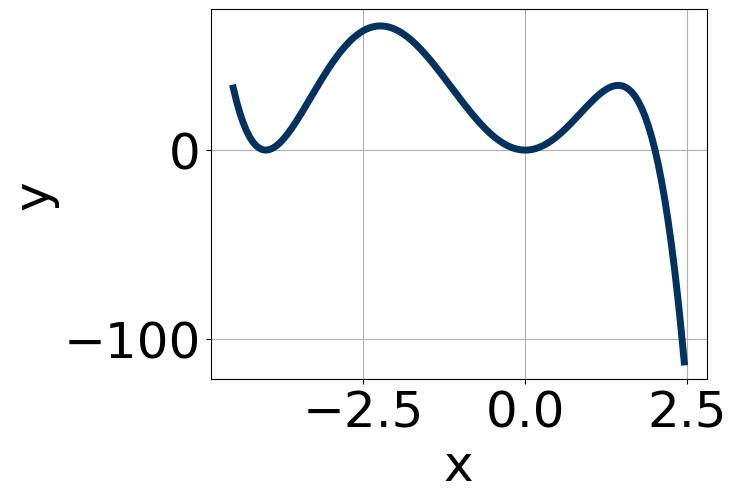
\includegraphics[width=0.5\textwidth]{../Figures/polyGraphToFunctionCopyC.png}
\end{center}
\begin{enumerate}[label=\Alph*.]
\item \( 11x^{11} (x + 4)^{7} (x + 1)^{5} \)
\item \( 17x^{6} (x + 4)^{4} (x + 1)^{9} \)
\item \( 9x^{4} (x + 4)^{7} (x + 1)^{7} \)
\item \( -15x^{6} (x + 4)^{7} (x + 1)^{11} \)
\item \( -9x^{9} (x + 4)^{5} (x + 1)^{5} \)

\end{enumerate} }
\litem{
Which of the following equations \textit{could} be of the graph presented below?
\begin{center}
    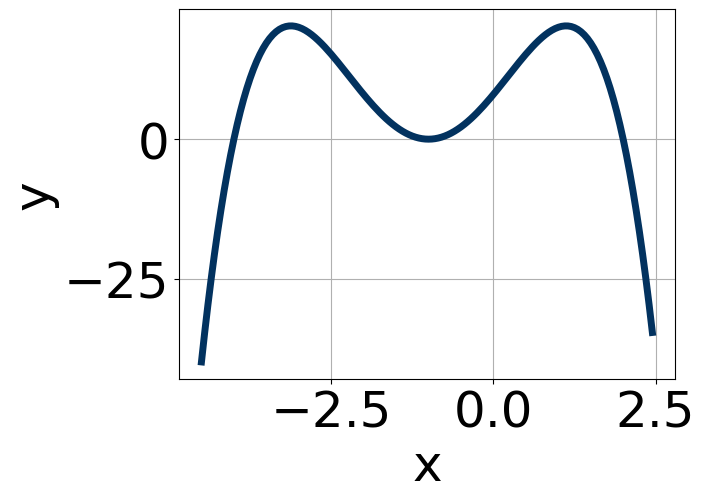
\includegraphics[width=0.5\textwidth]{../Figures/polyGraphToFunctionC.png}
\end{center}
\begin{enumerate}[label=\Alph*.]
\item \( -13(x + 1)^{8} (x + 2)^{10} (x - 3)^{9} \)
\item \( 11(x + 1)^{10} (x + 2)^{9} (x - 3)^{8} \)
\item \( 8(x + 1)^{6} (x + 2)^{7} (x - 3)^{5} \)
\item \( -20(x + 1)^{7} (x + 2)^{4} (x - 3)^{5} \)
\item \( -19(x + 1)^{4} (x + 2)^{7} (x - 3)^{7} \)

\end{enumerate} }
\litem{
Describe the zero behavior of the zero $x = -8$ of the polynomial below.\[ f(x) = 4(x - 8)^{9}(x + 8)^{10}(x + 6)^{7}(x - 6)^{10} \]\begin{enumerate}[label=\Alph*.]
\begin{multicols}{2}\item 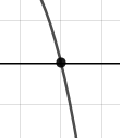
\includegraphics[width = 0.3\textwidth]{../Figures/polyZeroBehaviorAC.png}\item 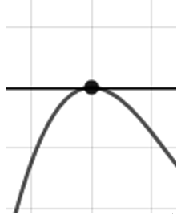
\includegraphics[width = 0.3\textwidth]{../Figures/polyZeroBehaviorBC.png}\item 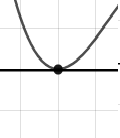
\includegraphics[width = 0.3\textwidth]{../Figures/polyZeroBehaviorCC.png}\item 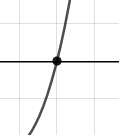
\includegraphics[width = 0.3\textwidth]{../Figures/polyZeroBehaviorDC.png}\end{multicols}\item None of the above.
\end{enumerate} }
\litem{
Describe the end behavior of the polynomial below.\[ f(x) = 2(x + 2)^{5}(x - 2)^{10}(x - 9)^{2}(x + 9)^{2} \]\begin{enumerate}[label=\Alph*.]
\begin{multicols}{2}\item 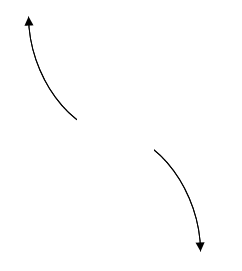
\includegraphics[width = 0.3\textwidth]{../Figures/polyEndBehaviorAC.png}\item 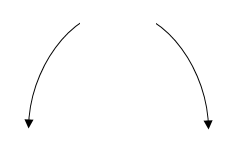
\includegraphics[width = 0.3\textwidth]{../Figures/polyEndBehaviorBC.png}\item 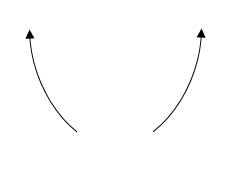
\includegraphics[width = 0.3\textwidth]{../Figures/polyEndBehaviorCC.png}\item 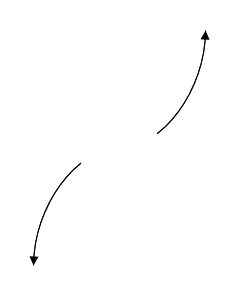
\includegraphics[width = 0.3\textwidth]{../Figures/polyEndBehaviorDC.png}\end{multicols}\item None of the above.
\end{enumerate} }
\litem{
Construct the lowest-degree polynomial given the zeros below. Then, choose the intervals that contain the coefficients of the polynomial in the form $ax^3+bx^2+cx+d$.\[ \frac{-7}{3}, -6, \text{ and } \frac{5}{4} \]\begin{enumerate}[label=\Alph*.]
\item \( a \in [7, 13], b \in [-121, -109], c \in [289, 294], \text{ and } d \in [-211, -202] \)
\item \( a \in [7, 13], b \in [85, 94], c \in [34, 46], \text{ and } d \in [209, 218] \)
\item \( a \in [7, 13], b \in [-85, -83], c \in [34, 46], \text{ and } d \in [209, 218] \)
\item \( a \in [7, 13], b \in [85, 94], c \in [34, 46], \text{ and } d \in [-211, -202] \)
\item \( a \in [7, 13], b \in [27, 37], c \in [-225, -220], \text{ and } d \in [209, 218] \)

\end{enumerate} }
\litem{
Construct the lowest-degree polynomial given the zeros below. Then, choose the intervals that contain the coefficients of the polynomial in the form $ax^3+bx^2+cx+d$.\[ \frac{-7}{3}, \frac{-5}{2}, \text{ and } -5 \]\begin{enumerate}[label=\Alph*.]
\item \( a \in [3, 13], b \in [-2, 3], c \in [-114, -105], \text{ and } d \in [172, 177] \)
\item \( a \in [3, 13], b \in [-61, -58], c \in [176, 187], \text{ and } d \in [-181, -166] \)
\item \( a \in [3, 13], b \in [29, 32], c \in [-38, -26], \text{ and } d \in [-181, -166] \)
\item \( a \in [3, 13], b \in [53, 69], c \in [176, 187], \text{ and } d \in [-181, -166] \)
\item \( a \in [3, 13], b \in [53, 69], c \in [176, 187], \text{ and } d \in [172, 177] \)

\end{enumerate} }
\litem{
Construct the lowest-degree polynomial given the zeros below. Then, choose the intervals that contain the coefficients of the polynomial in the form $x^3+bx^2+cx+d$.\[ 5 - 3 i \text{ and } 3 \]\begin{enumerate}[label=\Alph*.]
\item \( b \in [-16, -10], c \in [56, 67], \text{ and } d \in [-110, -98] \)
\item \( b \in [7, 16], c \in [56, 67], \text{ and } d \in [99, 103] \)
\item \( b \in [-1, 2], c \in [-14, -7], \text{ and } d \in [12, 18] \)
\item \( b \in [-1, 2], c \in [0, 8], \text{ and } d \in [-10, -6] \)
\item \( \text{None of the above.} \)

\end{enumerate} }
\litem{
Describe the end behavior of the polynomial below.\[ f(x) = 5(x + 4)^{5}(x - 4)^{8}(x + 3)^{2}(x - 3)^{3} \]\begin{enumerate}[label=\Alph*.]
\begin{multicols}{2}\item 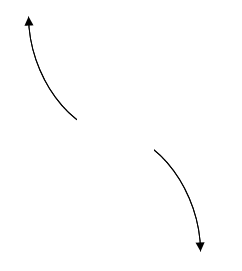
\includegraphics[width = 0.3\textwidth]{../Figures/polyEndBehaviorCopyAC.png}\item 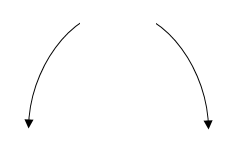
\includegraphics[width = 0.3\textwidth]{../Figures/polyEndBehaviorCopyBC.png}\item 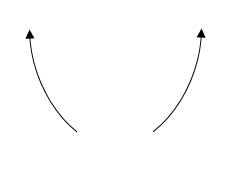
\includegraphics[width = 0.3\textwidth]{../Figures/polyEndBehaviorCopyCC.png}\item 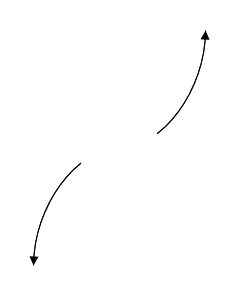
\includegraphics[width = 0.3\textwidth]{../Figures/polyEndBehaviorCopyDC.png}\end{multicols}\item None of the above.
\end{enumerate} }
\litem{
Describe the zero behavior of the zero $x = 8$ of the polynomial below.\[ f(x) = -7(x + 5)^{12}(x - 5)^{8}(x + 8)^{12}(x - 8)^{9} \]\begin{enumerate}[label=\Alph*.]
\begin{multicols}{2}\item 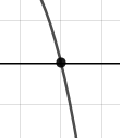
\includegraphics[width = 0.3\textwidth]{../Figures/polyZeroBehaviorCopyAC.png}\item 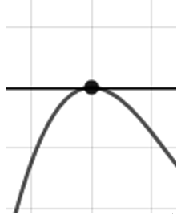
\includegraphics[width = 0.3\textwidth]{../Figures/polyZeroBehaviorCopyBC.png}\item 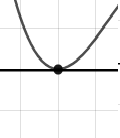
\includegraphics[width = 0.3\textwidth]{../Figures/polyZeroBehaviorCopyCC.png}\item 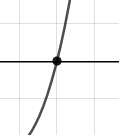
\includegraphics[width = 0.3\textwidth]{../Figures/polyZeroBehaviorCopyDC.png}\end{multicols}\item None of the above.
\end{enumerate} }
\litem{
Construct the lowest-degree polynomial given the zeros below. Then, choose the intervals that contain the coefficients of the polynomial in the form $x^3+bx^2+cx+d$.\[ 4 - 2 i \text{ and } -4 \]\begin{enumerate}[label=\Alph*.]
\item \( b \in [-3, 3.2], c \in [-4, 5], \text{ and } d \in [-21, -7] \)
\item \( b \in [1.5, 4.4], c \in [-12, -8], \text{ and } d \in [-82, -75] \)
\item \( b \in [-3, 3.2], c \in [1, 8], \text{ and } d \in [6, 13] \)
\item \( b \in [-5.7, -2.5], c \in [-12, -8], \text{ and } d \in [80, 83] \)
\item \( \text{None of the above.} \)

\end{enumerate} }
\end{enumerate}

\end{document}